\chapter{Proposta}\label{cap4}

\section{Usuários}

Pessoas e instituições estão se afastando cada vez mais de impressões e se aproximando de livros eletrônicos. Os e-books estão fazendo sucesso e estão cada vez mais sendo utilizado pelos editores para tornar disponíveis livros em formato eletrônico. Eles oferecem benefícios para os leitores incluindo a redução de danos ao meio ambiente, a portabilidade, o peso leve e ao reforço da capacidade de referência. Mas, para alguns leitores, e-books oferecem ainda mais: a sua primeira oportunidade de desfrutar da leitura. Essa pessoas com algum tipo de limitação, seja cego ou com baixa visão, pessoas com dislexia ou outras dificuldades de aprendizagem ou ainda que não conseguem segurar ou mudar a página de um livro encontram enormes dificuldades para ler livros impressos e, dependendo do caso, tal prática torna-se impossível \cite{chronicle}.

Neste contexto este mecanismo de semântica e ontologia proposto, poderia auxiliar os usuários de audiobooks a possuírem maior mobilidade e conforto ao dispor destas tecnologias.

\section{Terminologias Existentes}

\subsection{Tesauros}

\subsection{Ontologias Existente}


\section{Descrição do Ambiente Web}


\section{Cronograma}
A criação das atividades desse cronograma foram baseadas no plano de ensino da disciplina Tópicos especiais em Engenharia de Software. Este plano foi desenvolvido para o primeiro semestre letivo no ano de 2015.

 \begin{figure}[ht]
  \centering
    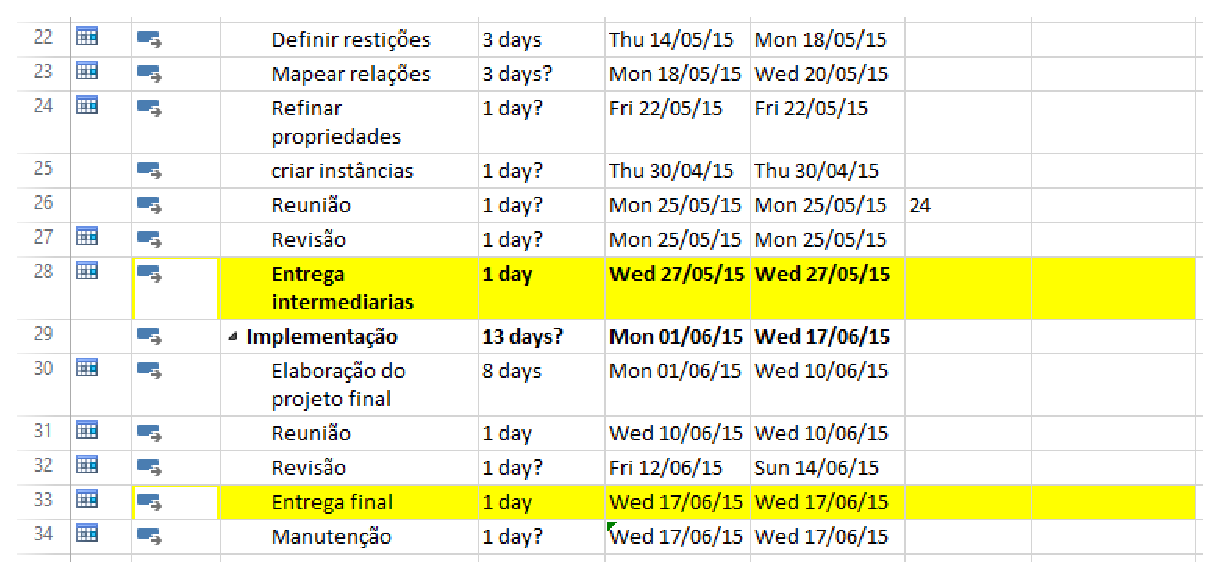
\includegraphics[keepaspectratio=true,scale=0.5]{figuras/cronograma.eps}
  \caption{Cronograma do projeto}
\end{figure}